\chapter{Attack vectors}
\label{chp:attack-vectors}

In this chapter, we describe several methods to gain control over a program vulnerable to stack buffer overflow attacks.
In each of the sections, it is assumed that none of the measures from \cref{chp:defense-mechanisms} are enabled or active unless otherwise stated.

% Differentiate between RIP and SFP overwriting? 
% If yes, in sections if applicable or in own section?
% What about overwriting data in general?
% Maybe own section at the end? Or somewhere in the middle?
%\section{Overwriting \glsentryshort{rip} and \glsentryshort{sfp}}

\section{Code injection}
\label{sec:code-injection}

\subsection{Operating principle}
\label{subsec:ci-operating-principle}

Code injection is the simplest attack vector for stack buffer overflows.
As described in \cref{sec:stack-buffer-overflows}, an attacker might try to overwrite the \gls{rip}.
If this is possible, an attacker can divert control flow to any location he wants.

At such locations, the attacker can place so-called \emph{shellcode} before overflowing the vulnerable buffer.
Shellcode is the binary representation of assembly instructions compiled to the corresponding \glspl{opcode}.
Such code can be directly executed by the processor without the need of compilation (high-level programming languages like C) or translating assembly instructions with an assembler.
Shellcode can be created by compiling the desired code or assembling the desired assembly instructions into an executable file.
The executable binary shellcode can then be extracted from the resulting binary file%
	\footnote{Public databases like \href{https://www.exploit-db.com/shellcodes}{exploit-db.com} already provide lots of pre-compiled shellcode suitable for different architectures and \glspl{os}.}%
.
The name \emph{shellcode} is derived from the general attacker's goal to spawn a shell and thus execute arbitrary commands.
However, shellcode can contain any instructions and does not necessarily have to spawn a shell on the attacked system directly.

\subsubsection{Code injection into the vulnerable buffer}
\label{subsubsec:ci-into-vuln-buffer}

One possibility for an attacker to execute shellcode is to place the shellcode into the buffer which is overflown before the \gls{rip} value, as they control the buffer's contents.
The return address then has to be overwritten with the address of the buffer on the stack.
If the right address is used, the program does not return to the caller function as intended but to the position on the stack where the overwritten buffer is located.
The processor then tries to decode the data on the stack as processor instructions and thus executes the shellcode stored in the buffer.

Such an attack is very hard to achieve correctly, as the return address written onto the stack has to match the buffer's address exactly.
An offset of the return address to the buffer's address of a single byte can already render the shellcode unusable, as the instructions are decoded incorrectly by the processor.
Thus, a common technique to improve the reliability of such an exploit is to include a so-called \emph{\gls{nop} sled} into the user-controlled input which is used to overflow the vulnerable buffer on the stack.
A \gls{nop} sled consists of binary encoded \acrshort{nop} assembly instructions (byte \texttt{0x90} on \texttt{x86/x86\_64}).
This instruction tells the processor to do nothing during the cycle where this instruction is executed.
If a lot of such instructions are placed in front of the shellcode into the buffer, the return address does not necessarily have to point exactly to the start of the buffer or the start of the shellcode but it is sufficient to point the return address to a location somewhere in the \acrshort{nop} sled.
When returning into the \acrshort{nop} sled, the processor then executes several \gls{nop} instructions and progresses on the stack until it reaches the shellcode.

It is also possible to place the \acrshort{nop} sled after the shellcode on the stack instead of in front of the shellcode.
If the length of the shellcode and the \acrshort{nop} sled is known, a relative jump can be added to the end of the \acrshort{nop} sled with the negative offset for the relative jump being the combined length of the shellcode and the \acrshort{nop} sled.
As shown in \cref{fig:stack-overflow-nop-sled}, such a \acrshort{nop} sled can even extend over the overwritten return address with the help of a second relative jump in order to bypass size restrictions given by the size of the buffer.

\begin{figure}[htb]
	\centering
	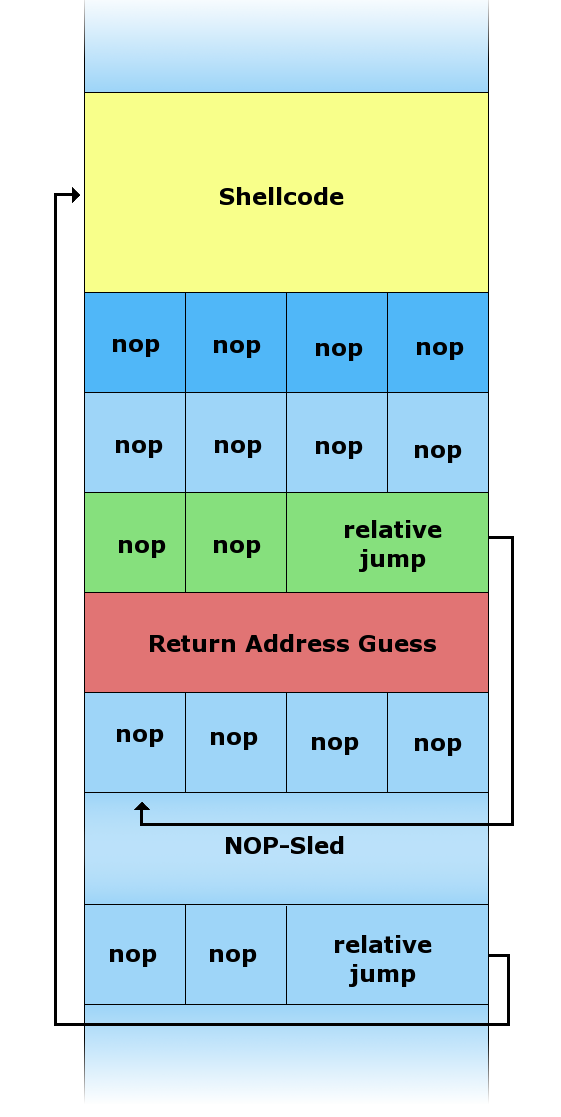
\includegraphics[width=0.3\textwidth]{figures/NopSled}
	\caption{Stack layout after a stack buffer overflow with shellcode and \acrshort{nop} sled \cite{Lynn2007c} (c.f. \cref{fig:stack-layout})}
	\label{fig:stack-overflow-nop-sled}
\end{figure}

In general, a long \acrshort{nop} sled is desired by an attacker, as it becomes easier to guess an address inside of the \acrshort{nop} sled \cite{AlephOne1996}.

\subsubsection{Code injection via environment variables}
\label{subsubsec:ci-via-env-variable}

If it is desired to have a contiguous block of shellcode with maybe a \acrshort{nop} sled in front of it without the necessity of relative jumps, it might be a problem to have the exploit code fit into the vulnerable buffer before the overwritten return address, as the buffer might be too small to store the whole input.
In such cases, the actual exploit code (\acrshort{nop} sled and shellcode) can be put into an environment variable on the system which is being attacked if the attacker has the necessary access to the system to set environment variables.
Environment variables are not restricted in size and are loaded onto the bottom of the stack on program startup \cite[731\psq]{Bryant2011}.

Thus, it is possible to point the return address into an environment variable instead of the overflown buffer.
If the return address successfully points either directly to the shellcode or into the \acrshort{nop} sled inside the environment variable, the shellcode is executed exactly as in the previous case where it was put into the user-controlled overflown buffer.

A restriction of this approach is that environment variables are only mapped into the processes address space when the process is started.
Thus, shellcode cannot be injected into already running programs with the help of environment variables but only into programs started after setting the environment variable.

\subsubsection{Code injection into global variables}
\label{subsubsec:ci-via-globals}

\subsubsection{Code injection into arbitrary buffers}
\label{subsubsec:ci-into-arbitrary-buffer}

\subsection{Countermeasures}
\label{subsec:ci-countermeasures}

\begin{itemize}
	\item{\gls{nx} bit}
	\item{\gls{aslr}}
\end{itemize}



\begin{itemize}
	\item{Shellcode injection}
	\item{Position independent shellcode}
	\item{NOP sled}
\end{itemize}

\section{Returning into executable code}
\label{sec:returning-into-executable-code}

\subsection{\Glsentrylong{ret2libc} (\glsentryshort{ret2libc})}
\label{subsec:ret2libc}

\subsection{\glsentrylong{rop} (\glsentryshort{rop})}
\label{subsec:rop}

\subsection{\glsentrylong{jop} (\glsentryshort{jop})}
\label{subsec:jop}

\subsection{\glsentrylong{cop} (\glsentryshort{cop})}
\label{subsec:cop}
